\documentclass{article}


% Useful libraries
%%%%%%%%%%%%%%%%%%%%%%%%%%%%%%%%%%%%%%%%%%%%%%%%%%%%%%%%%%%%%%%%%%%%%%%%%%%%%%%
\usepackage[noend]{algpseudocode}
\usepackage{amsmath, amssymb, mathtools}
\usepackage{algorithmicx}
\usepackage{algorithm}
\usepackage{amsmath}
\usepackage{pgfplots}
\usepackage{setspace}
\usepackage{subfig}
\usepackage{tabularx}

\usetikzlibrary{arrows.meta}
\usetikzlibrary{arrows}
\usetikzlibrary{backgrounds}
\usetikzlibrary{calc}
\usetikzlibrary{fit}
\usetikzlibrary{positioning}
\usetikzlibrary{shapes}

\usepackage[
	pagebackref=false,
	colorlinks,
	linkcolor=blue,
	citecolor=blue,
	urlcolor=blue
]{hyperref}



\def\imgscale{0.23}



%%%%%%%%%%%%%%%%%%%%%%%%%%%%%%%%%%%%%%%%%%%%%%%%%%%%%%%%%%%%%%%%%%%%%%%%%%%%%%%
\begin{document}

\title{How To Build ILI9325 TFT LCD Component for Proteus VSM}
\author{Vahid Heidari}
\date{\today}
\maketitle



%%%%%%%%%%%%%%%%%%%%%%%%%%%%%%%%%%%%%%%%%%%%%%%%%%%%%%%%%%%%%%%%%%%%%%%%%%%%%%%
\section{Introduction}

\texttt{Proteus VSM} is an electronic circuit simulator best known for its reach
digital component library. It comes with a CAD program, named \texttt{ARES},
that allows you to design PCB boards based on schematics.

Unfortunately, \texttt{Proteus} does not have any \texttt{ILI9325} TFT LCD
component. The only way to simulate this component is to provide a custom-made
library. In this project, thanks to \texttt{Proteus VSM} C++ SDK, I wrote an
\texttt{ILI9325} library.

In this article, I explain the process of designing a 2D graphical
representation, building a \texttt{.DLL} module for handling active digital
model, and installing this user build component to \texttt{Proteus VSM} for
simulation.



%%%%%%%%%%%%%%%%%%%%%%%%%%%%%%%%%%%%%%%%%%%%%%%%%%%%%%%%%%%%%%%%%%%%%%%%%%%%%%%
\section{Designing 2D Graphical Representation}

Select \texttt{2D Graphics Box Mode} tool from the left side tool bar and draw a
rectangle as a base of the LCD panel.
\begin{figure}[!ht]
\centering
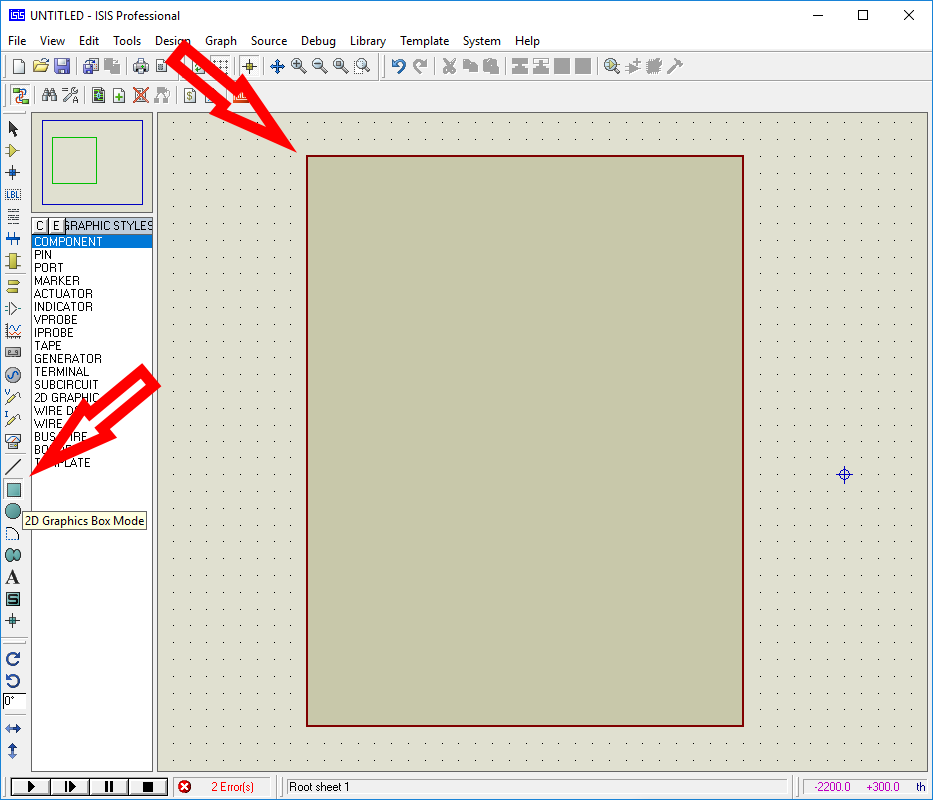
\includegraphics [scale=\imgscale] {Images/01-base/0-2d-box.png}
\end{figure}


%%%%%%%%%%%%%%%%%%%%%%%%%%%%%%%%%%%%%%%%

Then select \texttt{Device Pin Mode} and put a pin (orient the pin if needed).
Right click on the pin and select \texttt{Edit Properties} from the drop down
menu to open the \texttt{Edit Pin} dialog. Type the name of the and number of
the pin, and check the \texttt{IP - Input} option.

\begin{figure}[!ht]
\centering
\subfloat {
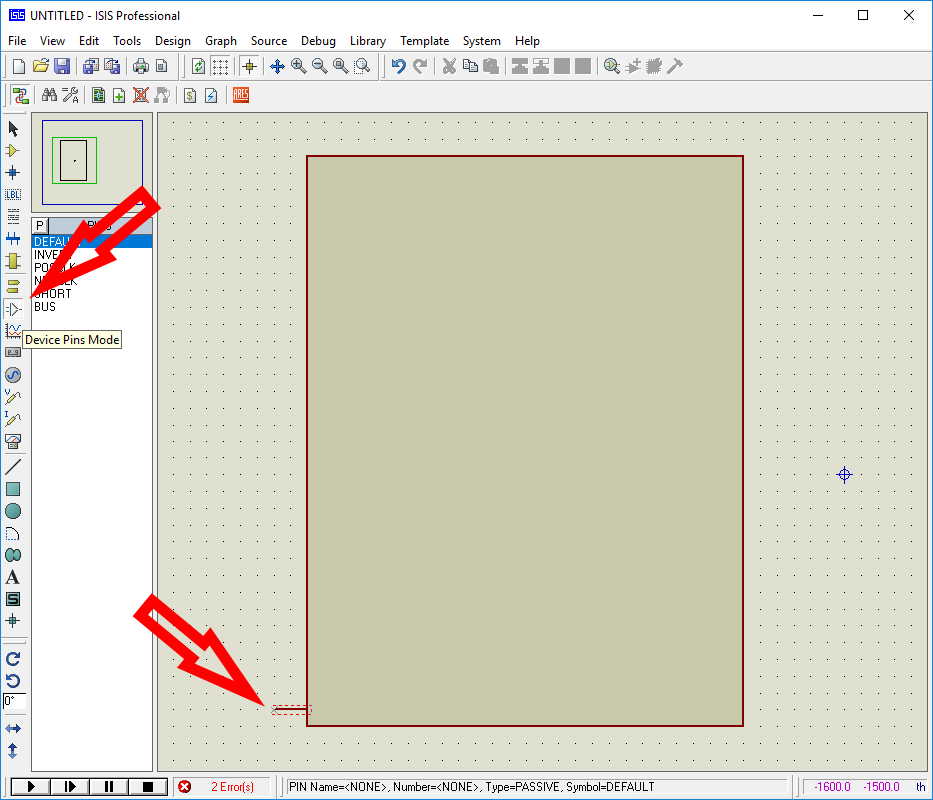
\includegraphics [scale=\imgscale] {Images/02-pins/0-device-pin-mode.png}
} \subfloat {
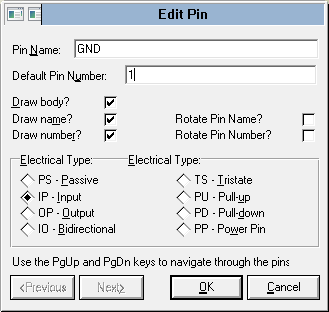
\includegraphics [scale=\imgscale] {Images/02-pins/1-pins-GND-edit.png}
}
\end{figure}


Repeat the previous steps for all other pins.

\begin{figure}[!ht]
\centering
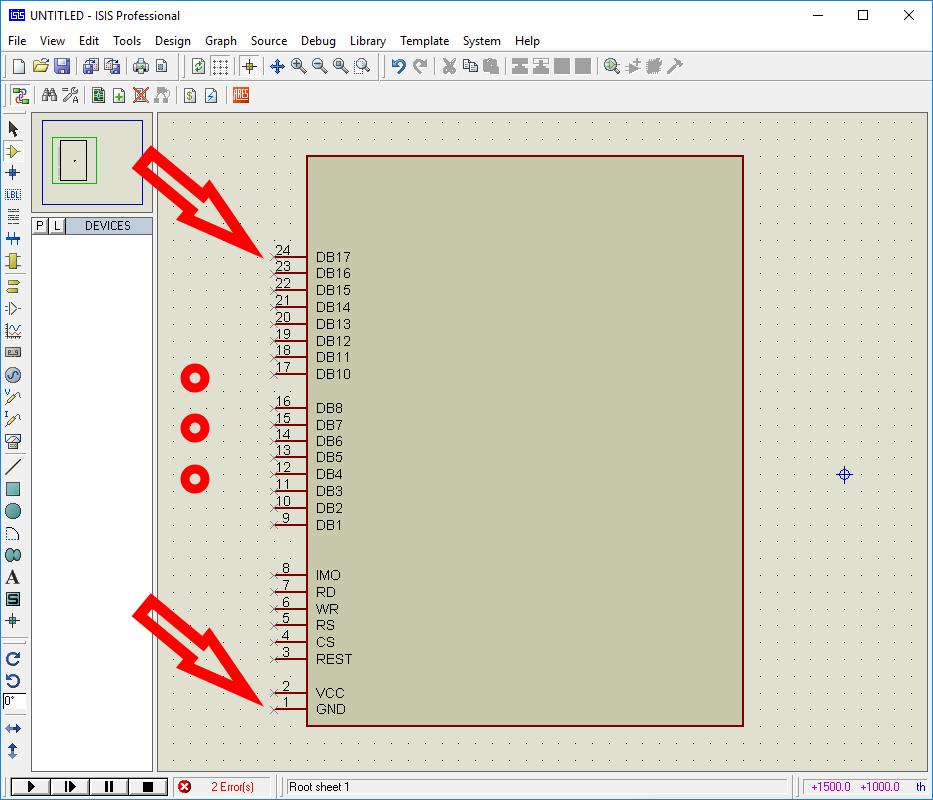
\includegraphics [scale=\imgscale] {Images/02-pins/2-pins.png}
\end{figure}


Check \texttt{IO - Bidirectional} option for \texttt{DB1} to \texttt{DB17} as
shown in the picture.

\begin{figure}[!ht]
\centering
\subfloat {
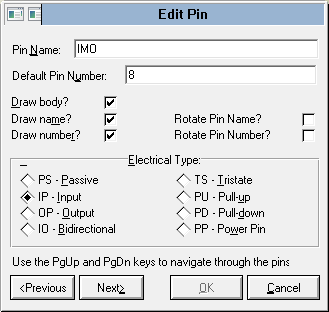
\includegraphics [scale=\imgscale] {Images/02-pins/3-pins-in-edit.png}
} \subfloat {
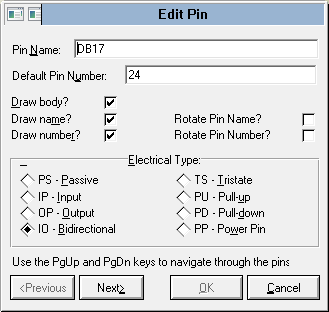
\includegraphics [scale=\imgscale] {Images/02-pins/4-pins-edit.png}
}
\end{figure}



%%%%%%%%%%%%%%%%%%%%%%%%%%%%%%%%%%%%%%%%

\newpage
Go back to \texttt{2D Graphics Box Mode} and draw another rectangle for the
bezel frame and change its color and border line as shown in the picture.

\begin{figure}[!ht]
\centering
\subfloat {
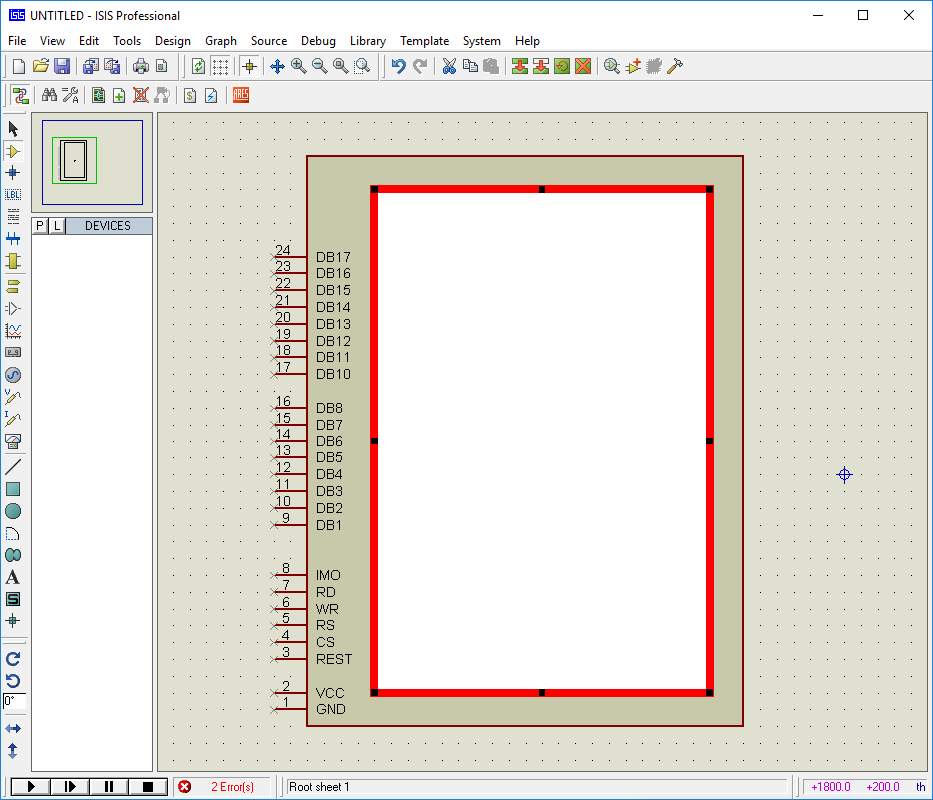
\includegraphics [scale=\imgscale] {Images/03-panel/0-marker1.png}
} \subfloat {
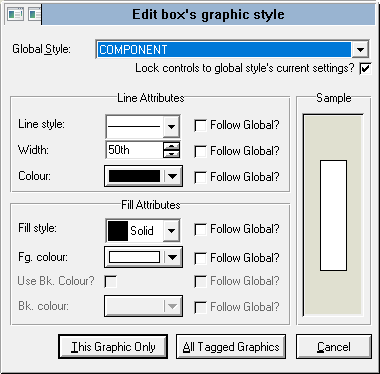
\includegraphics [scale=\imgscale] {Images/03-panel/1-marker1-edit.png}
} \\
\subfloat {
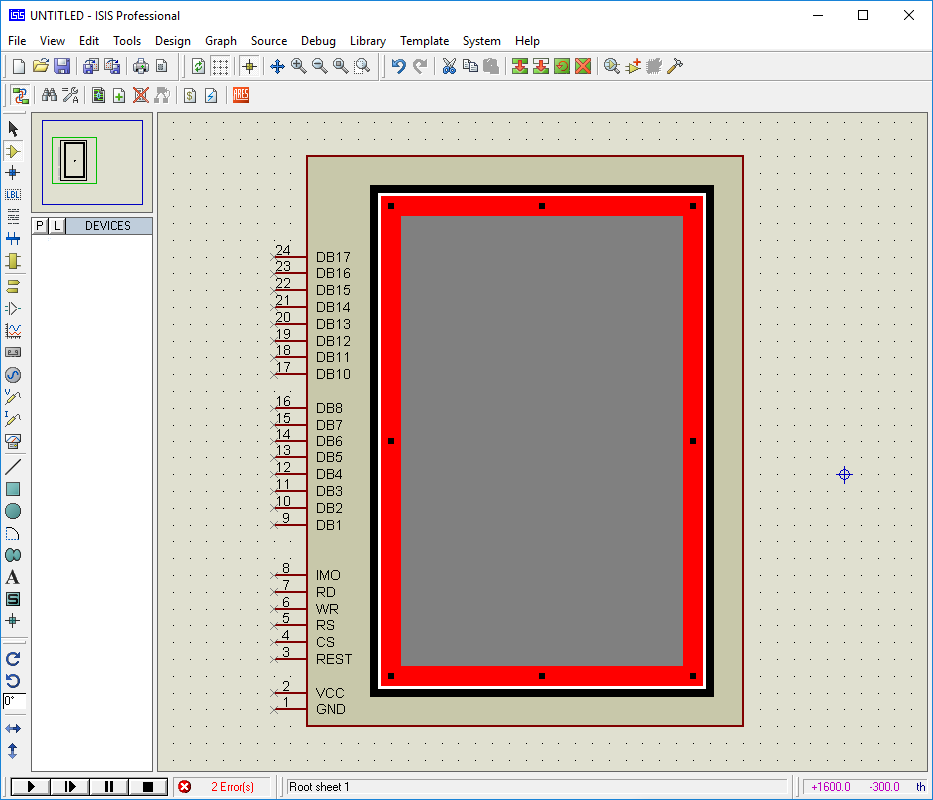
\includegraphics [scale=\imgscale] {Images/03-panel/2-marker2.png}
} \subfloat {
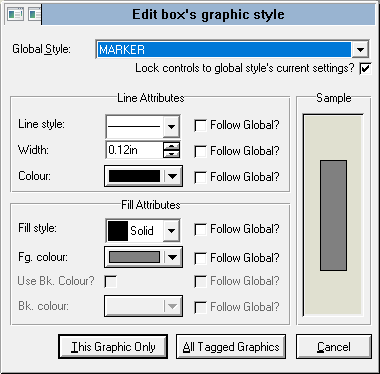
\includegraphics [scale=\imgscale] {Images/03-panel/3-marker2-edit.png}
}
\end{figure}


Draw the TFT glass on top of bezel frame. This rectangle is the actual drawing
area that is filled with pixel colors in code.

\begin{figure}[!ht]
\centering
\subfloat {
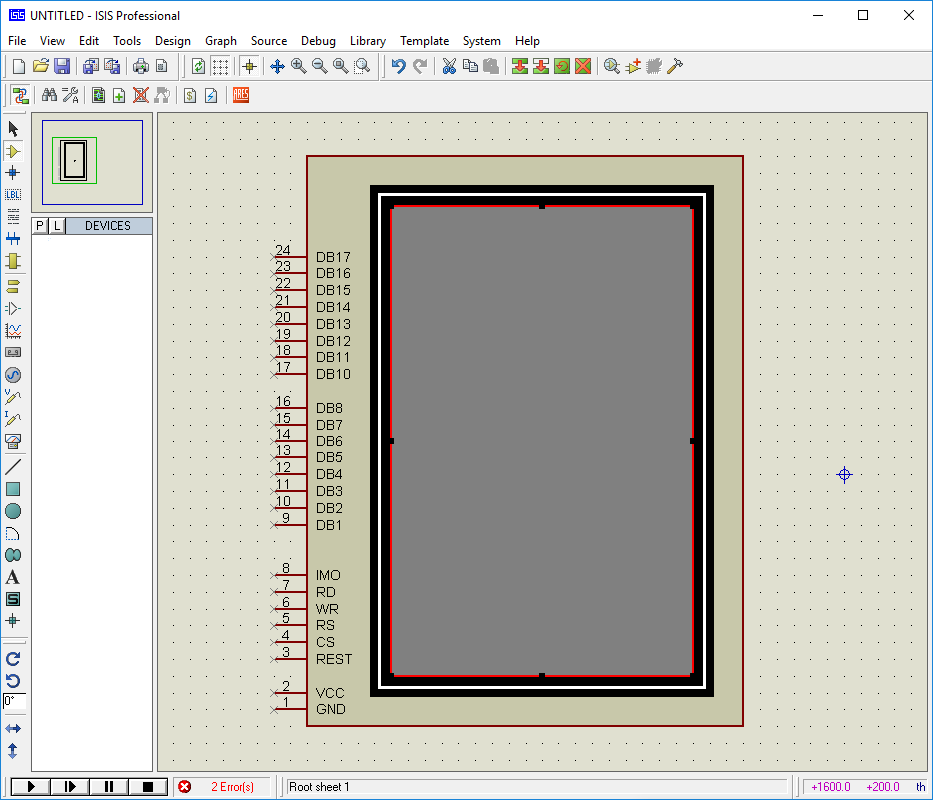
\includegraphics [scale=\imgscale] {Images/03-panel/4-lcd-area.png}
} \subfloat {
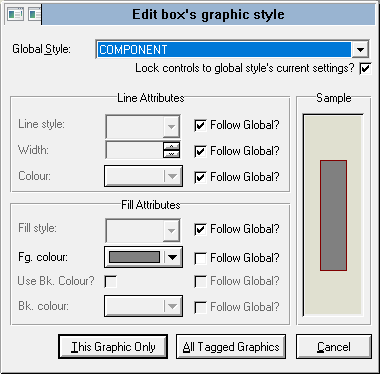
\includegraphics [scale=\imgscale] {Images/03-panel/5-lcd-area-edit.png}
}
\end{figure}


Select \texttt{2D Graphics Markers Mode} and place a \texttt{ORGIN} marker in
the center of the TFT glass.

\begin{figure}[!ht]
\centering
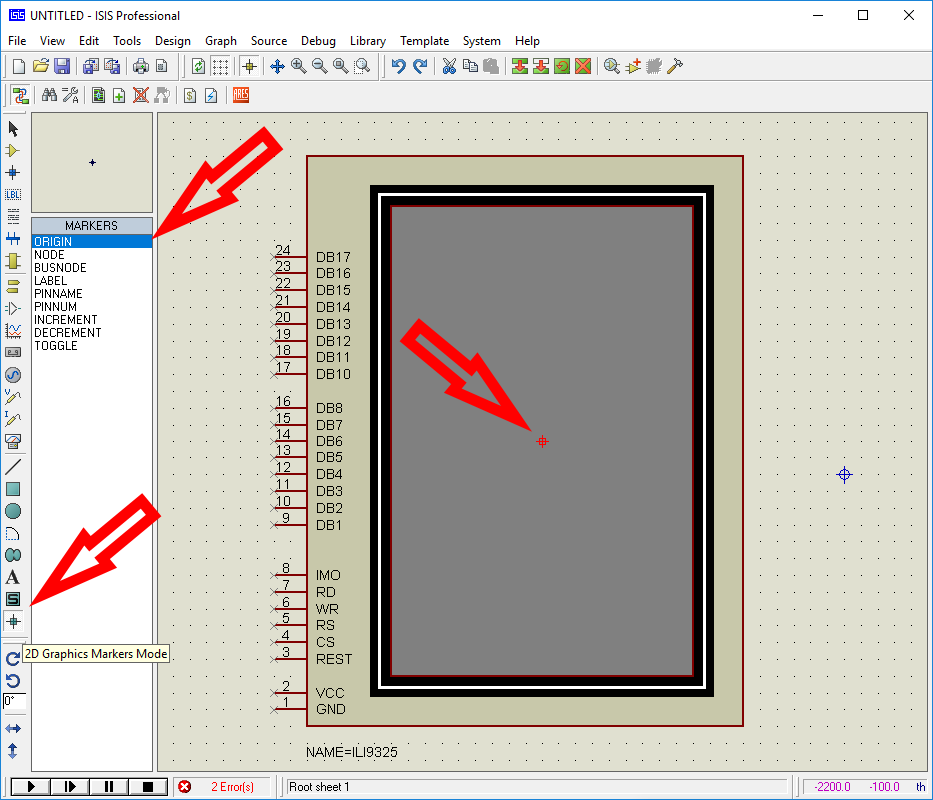
\includegraphics [scale=\imgscale] {Images/03-panel/6-orgin-marker.png}
\end{figure}


Now our graphical representation of the LCD is completed.

\begin{figure}[!ht]
\centering
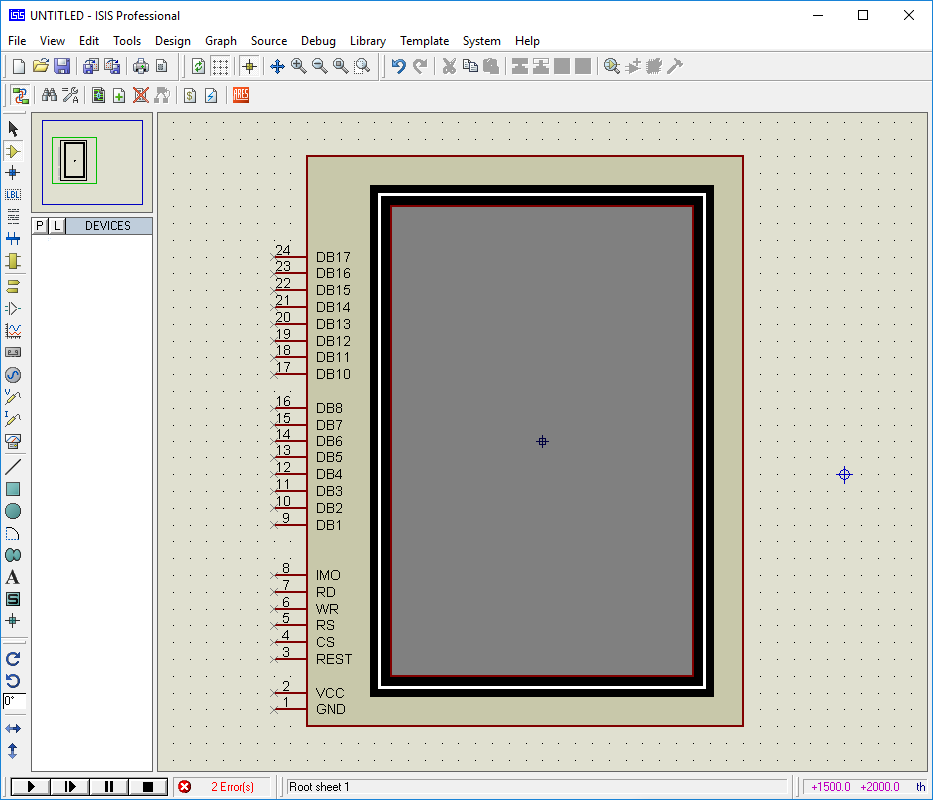
\includegraphics [scale=\imgscale] {Images/03-panel/7-2d-cmplt.png}
\end{figure}



%%%%%%%%%%%%%%%%%%%%%%%%%%%%%%%%%%%%%%%%

\newpage
Select the whole elements and right click. From the drop down menu select
\texttt{Make Device}.

\begin{figure}[!ht]
\centering
\subfloat {
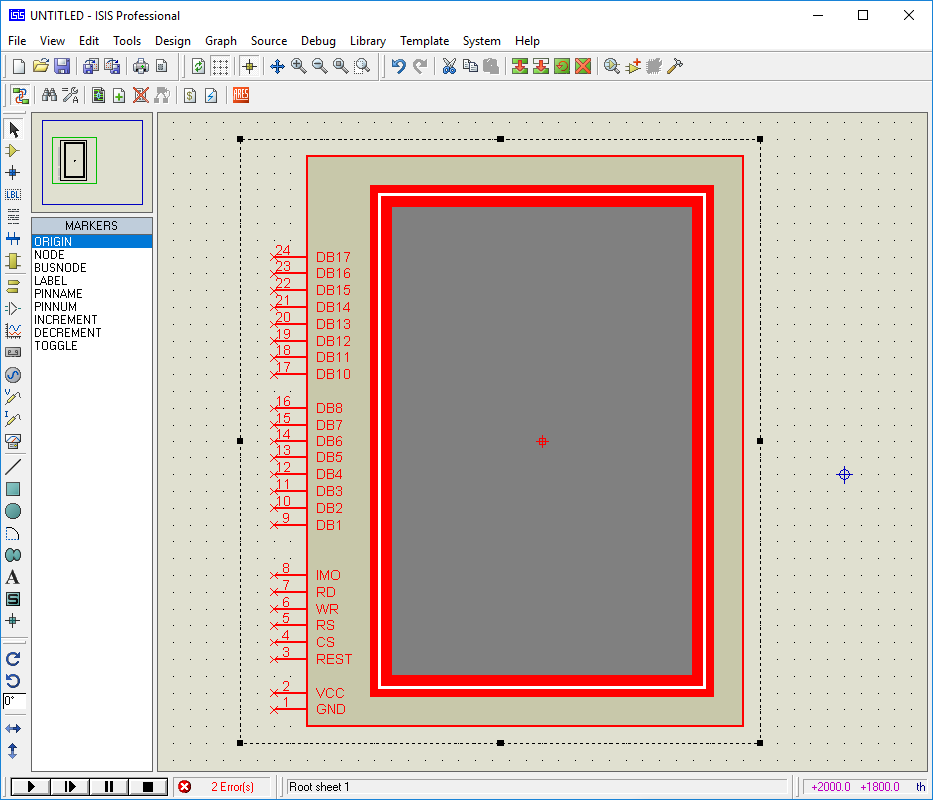
\includegraphics [scale=\imgscale] {Images/04-make-device/0-select-all.png}
} \subfloat {
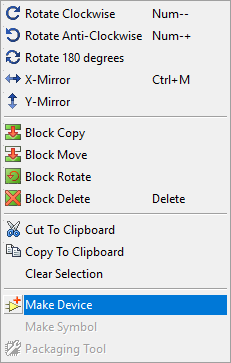
\includegraphics [scale=\imgscale] {Images/04-make-device/1-make-device.png}
}
\end{figure}



%%%%%%%%%%%%%%%%%%%%%%%%%%%%%%%%%%%%%%%%
\newpage
Fill the text-boxes as shown in the picture and click \texttt{Next} button.

\begin{figure}[!ht]
\centering
\subfloat {
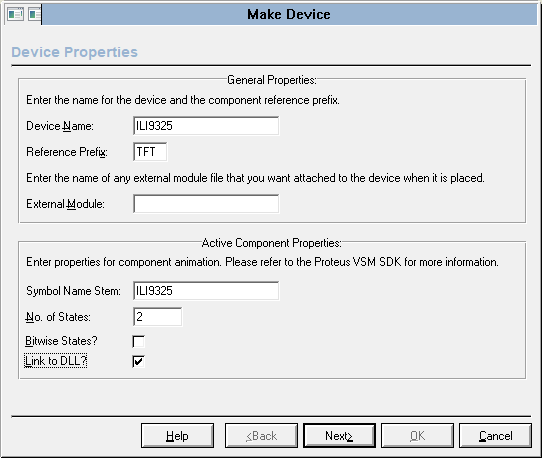
\includegraphics [scale=\imgscale] {Images/04-make-device/make-device-dg-1.png}
} \subfloat {
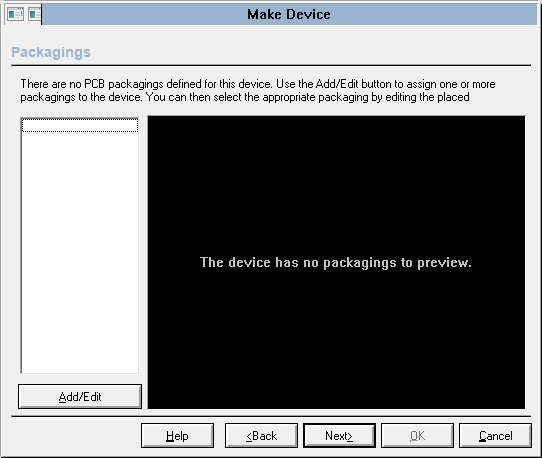
\includegraphics [scale=\imgscale] {Images/04-make-device/make-device-dg-2.png}
} \\ %%%%%%%%%%%%%%%%%%%%%%%%%%%%%%%%%%%%%%%%
\subfloat {
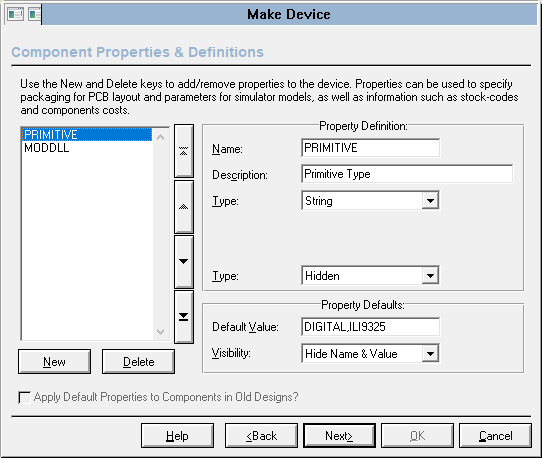
\includegraphics [scale=\imgscale] {Images/04-make-device/make-device-dg-3.png}
} \subfloat {
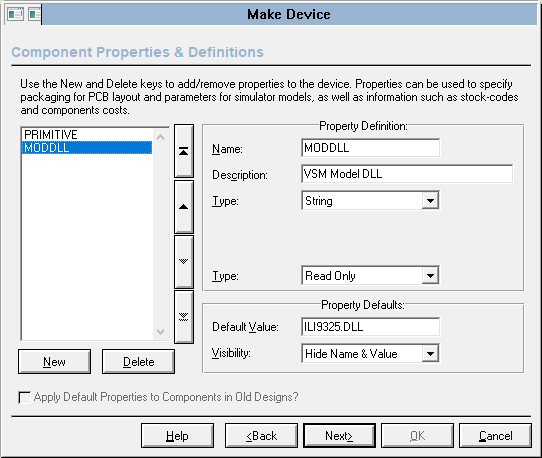
\includegraphics [scale=\imgscale] {Images/04-make-device/make-device-dg-4.png}
} \\ %%%%%%%%%%%%%%%%%%%%%%%%%%%%%%%%%%%%%%%%
\subfloat {
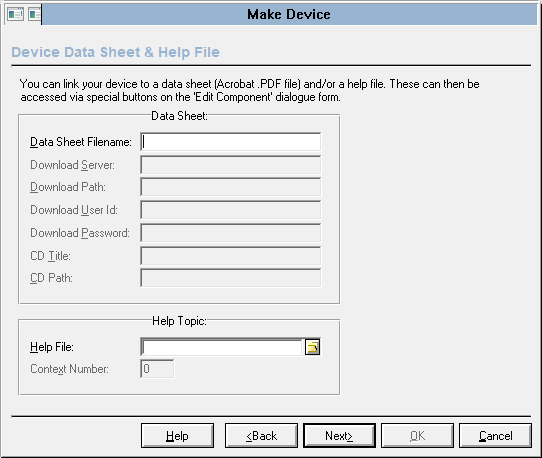
\includegraphics [scale=\imgscale] {Images/04-make-device/make-device-dg-5.png}
} \subfloat {
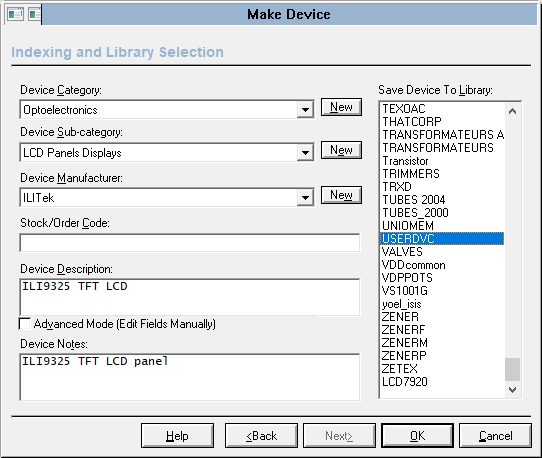
\includegraphics [scale=\imgscale] {Images/04-make-device/make-device-dg-6.png}
}
\end{figure}


In the last dialog, click \text{OK} to add the \texttt{ILI9325} device to the
\texttt{Proteus} library. You can select the device by searching from the
\texttt{Pick Devices} menu and place it in design sheet.



\clearpage
\newpage
%%%%%%%%%%%%%%%%%%%%%%%%%%%%%%%%%%%%%%%%%%%%%%%%%%%%%%%%%%%%%%%%%%%%%%%%%%%%%%%
\section{Making Symbols}

\texttt{Proteus} uses symbols to animate active components. In this project we
make two symbols for \texttt{ILI9325} LCD panel. Select \texttt{ILI9325}
component form \texttt{Pick Devices} menu.

\begin{figure}[!ht]
\centering
\subfloat {
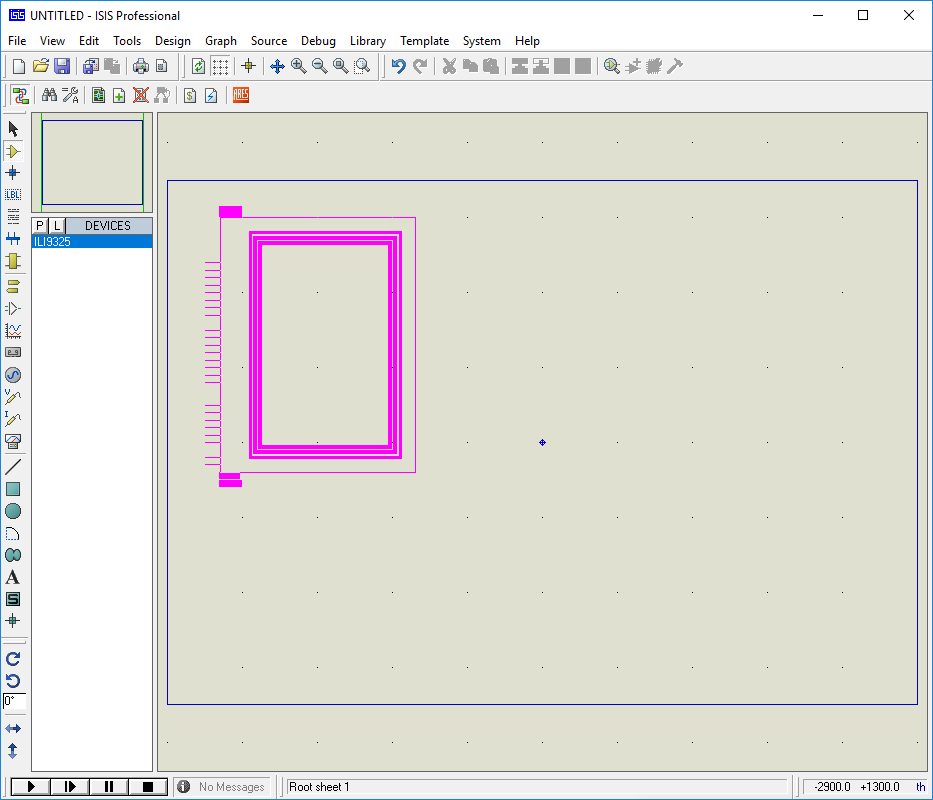
\includegraphics [scale=\imgscale] {Images/05-symbols/0-pickdevice.png}
} \subfloat {
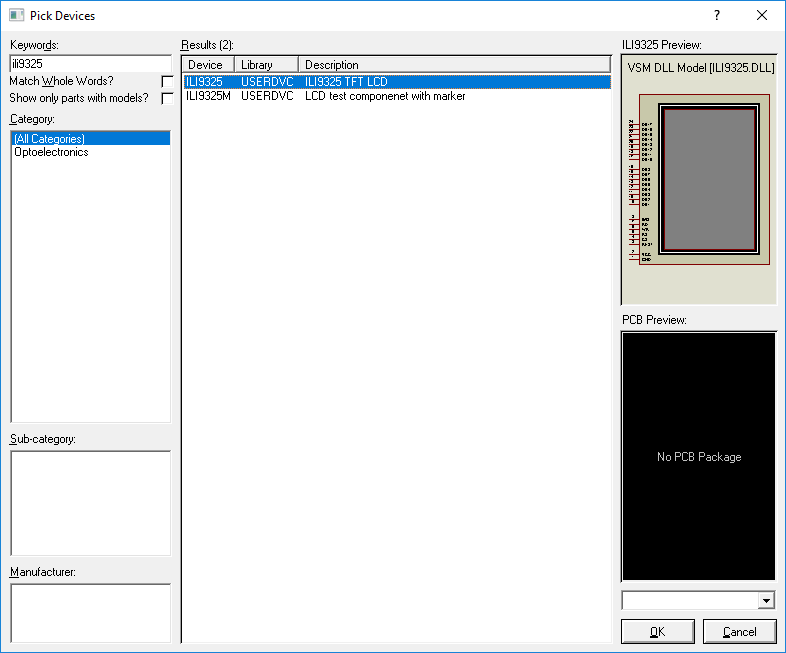
\includegraphics [scale=\imgscale] {Images/05-symbols/1-search.png}
}
\end{figure}


Place a LCD on the design sheet. Right click on the component and select the
\texttt{Decompose} option from the menu.

\begin{figure}[!ht]
\centering
\subfloat {
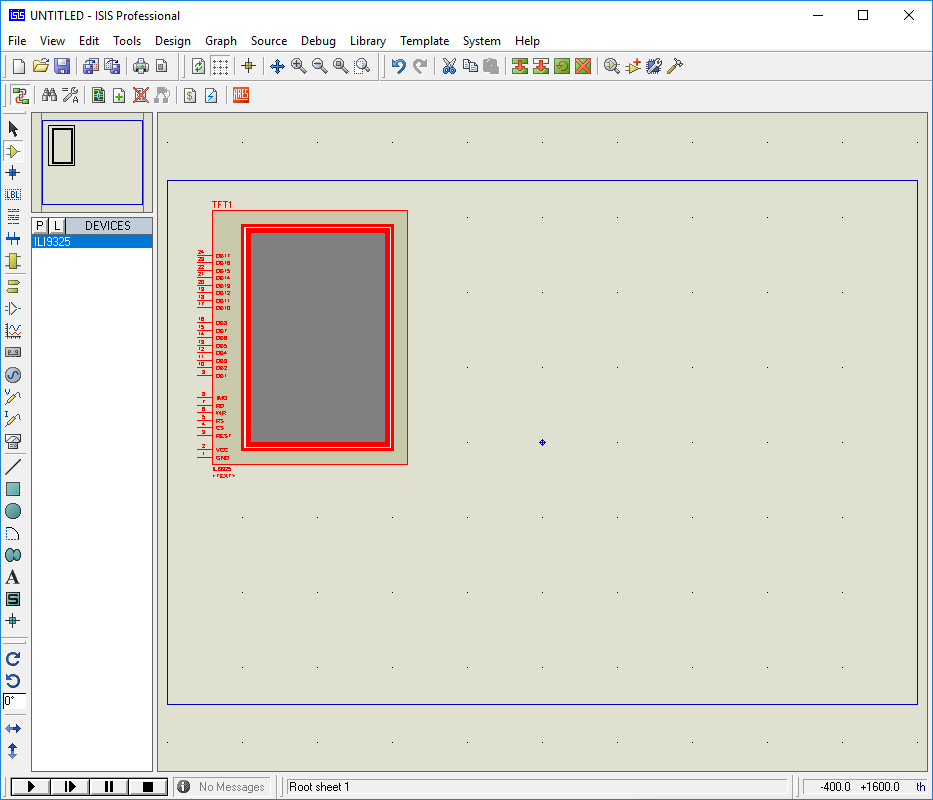
\includegraphics [scale=\imgscale] {Images/05-symbols/2-insert.png}
} \subfloat {
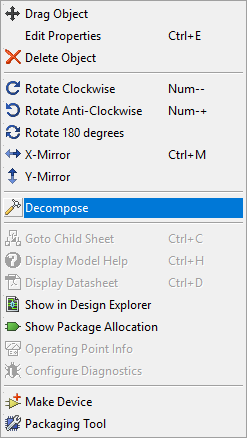
\includegraphics [scale=\imgscale] {Images/05-symbols/3-decompose.png}
}
\end{figure}


\newpage
Delete all part of the LCD except TFT glass and \texttt{ORIGIN} marker, then
block copy another instance.

\begin{figure}[!ht]
\centering
\subfloat {
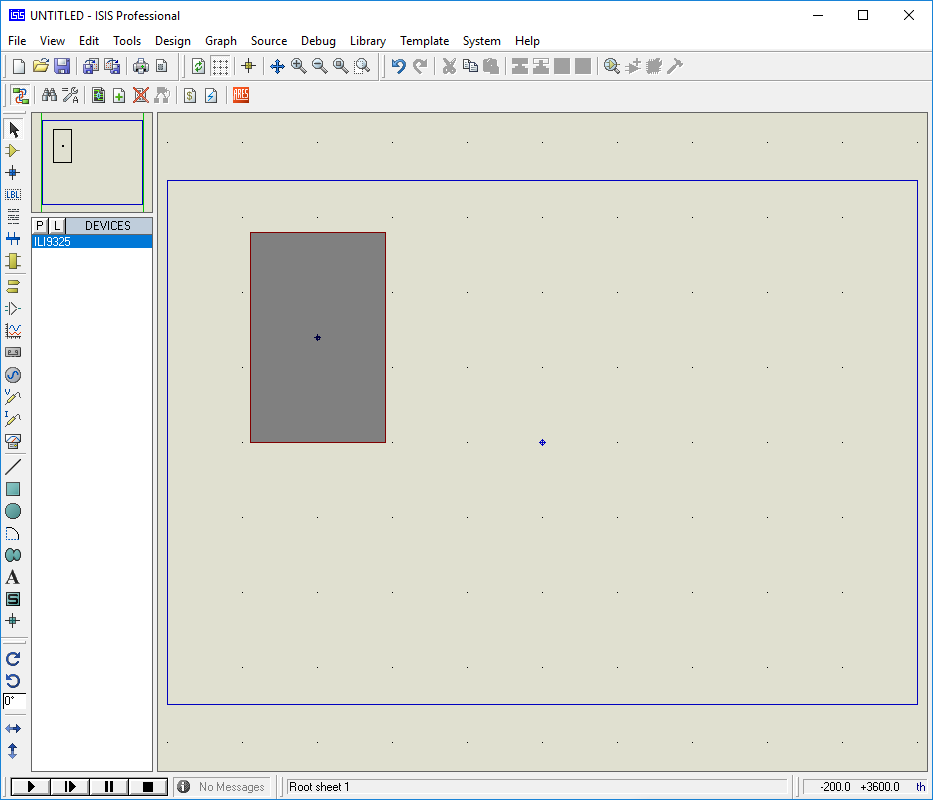
\includegraphics [scale=\imgscale] {Images/05-symbols/4-blockcopy.png}
} \subfloat {
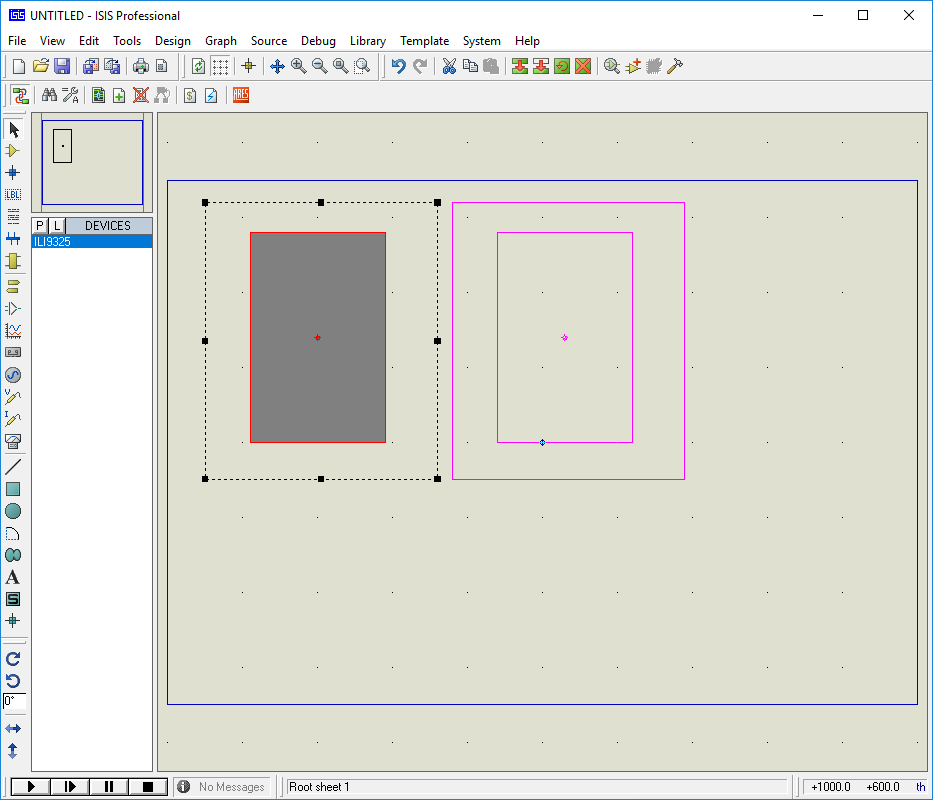
\includegraphics [scale=\imgscale] {Images/05-symbols/5-2copy.png}
}
\end{figure}


Select the first rectangle and change its color by right clicking on it and
selecting \texttt{Edit Properties}. Uncheck the \texttt{follow Global?} check
box and change the \texttt{Fg. colour} option from the color picker menu, then
click on \texttt{This Graphic Only} button.

\begin{figure}[!ht]
\centering
\subfloat {
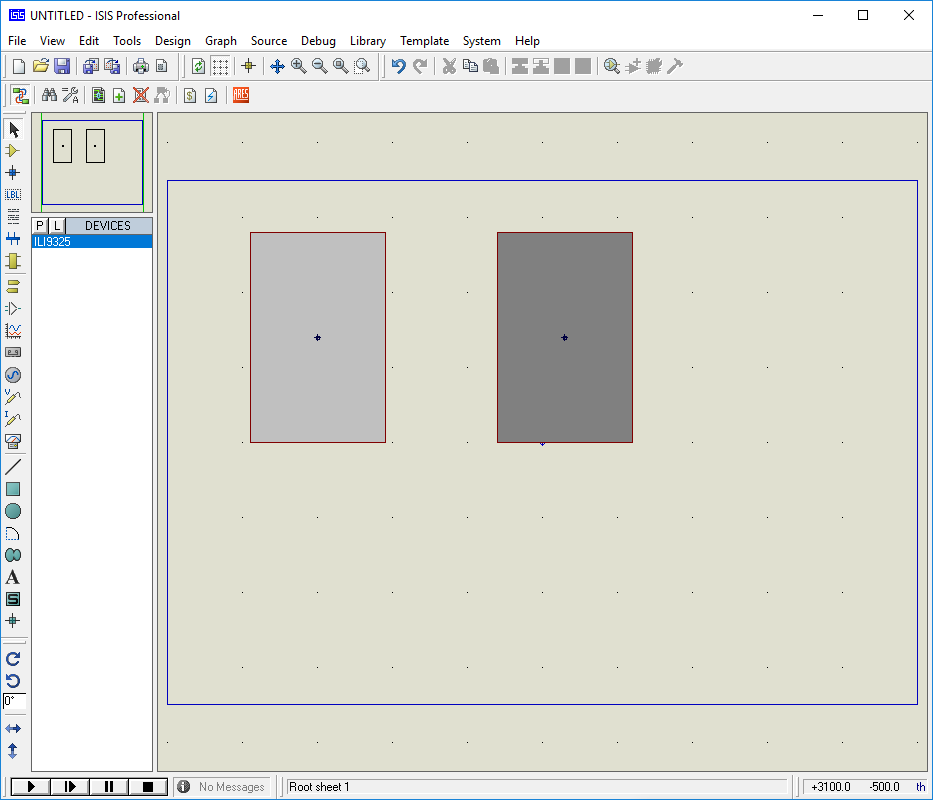
\includegraphics [scale=\imgscale] {Images/05-symbols/6-1-sym-color.png}
} \subfloat {
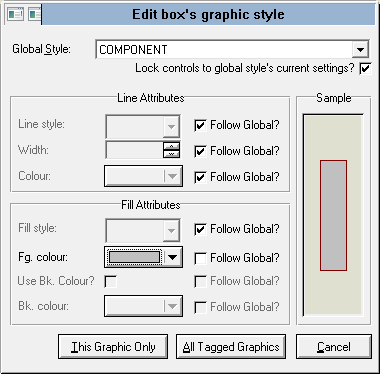
\includegraphics [scale=\imgscale] {Images/05-symbols/6-2-component.png}
} \subfloat {
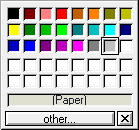
\includegraphics [scale=\imgscale] {Images/05-symbols/6-3-color-picker.png}
} \subfloat {
}
\end{figure}


\newpage
Do the same steps for the next rectangle but change its color to white.

\begin{figure}[!ht]
\centering
\subfloat {
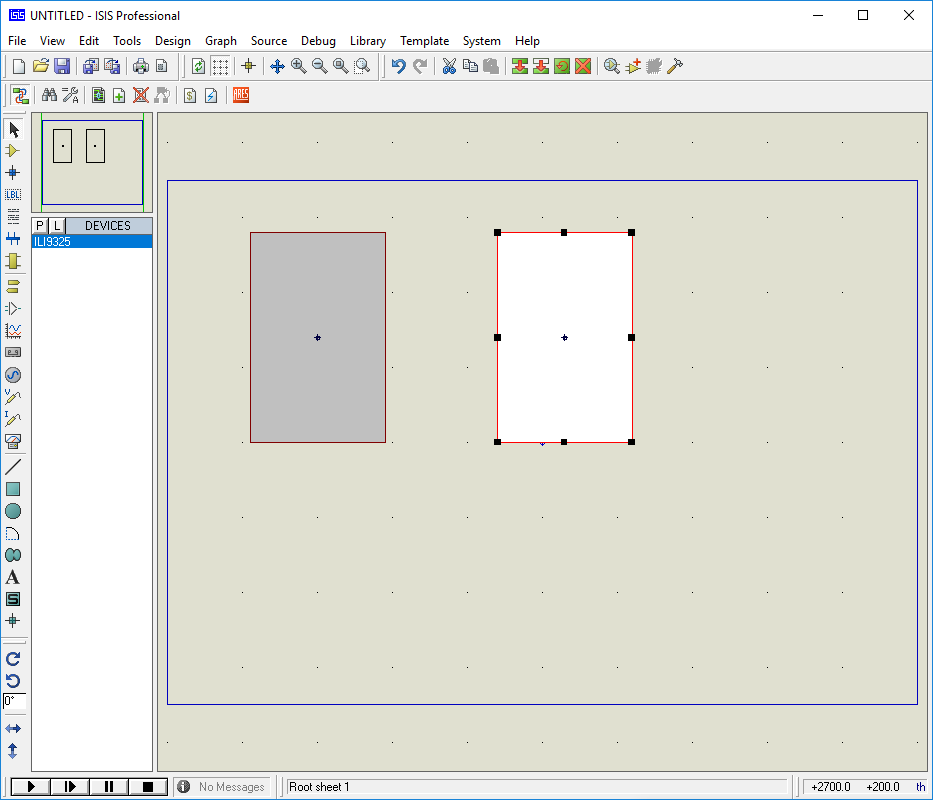
\includegraphics [scale=\imgscale] {Images/05-symbols/7-1-sym-color.png}
} \subfloat {
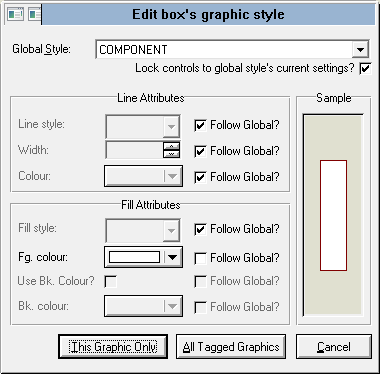
\includegraphics [scale=\imgscale] {Images/05-symbols/7-2-this-graphic-only.png}
} \subfloat {
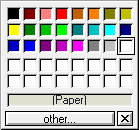
\includegraphics [scale=\imgscale] {Images/05-symbols/7-3-color.png}
}
\end{figure}


Select the first rectangle and \texttt{ORIGIN} marker and right click. From the
menu, select \texttt{Make Symbol} option. Take care that the symbol name MUST
follow the \texttt{Symbol Name Stem} pattern from the \texttt{Make Device}
dialog.

\begin{figure}[!ht]
\centering
\subfloat {
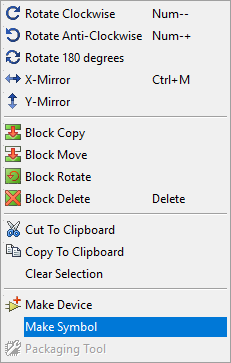
\includegraphics [scale=\imgscale] {Images/05-symbols/8-1-make-symbol.png}
} \subfloat {
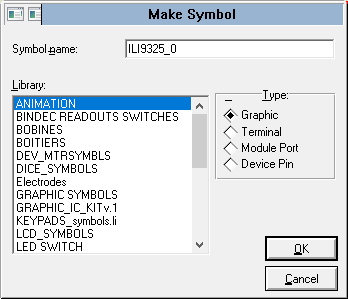
\includegraphics [scale=\imgscale] {Images/05-symbols/8-2-make-symobl-0.png}
}
\end{figure}


For the second symbol do the same steps and type \texttt{Symbol name} as
follows.

\begin{figure}[!ht]
\centering
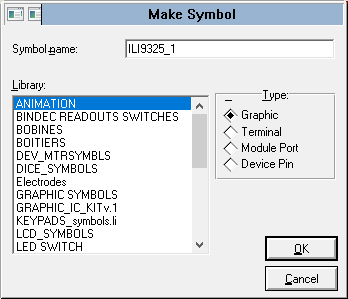
\includegraphics [scale=\imgscale] {Images/05-symbols/9-make-symbol-2.png}
\end{figure}

You can check the addition of symbols by searching in \texttt{Pick Symbols} form
the \texttt{2D Graphics Symbols Mode} on side panel.


\clearpage
\newpage
%%%%%%%%%%%%%%%%%%%%%%%%%%%%%%%%%%%%%%%%%%%%%%%%%%%%%%%%%%%%%%%%%%%%%%%%%%%%%%%
\section{Building \texttt{.DLL} Module}

Making \texttt{.DLL} module is strait forward. You can follow instructions from 
\texttt{Proteus VSM} SDK documentation \cite{VSMSDK}, section VSM MODELLING
TUTORIAL. I also found a useful Github repository \cite{LCD12864}. The only note 
you should take care of is you MUST make a 32-bit \texttt{.DLL} because
\texttt{Proteus} does not recognize 64-bit \text{.DLL}s.


%%%%%%%%%%%%%%%%%%%%%%%%%%%%%%%%%%%%%%%%%%%%%%%%%%%%%%%%%%%%%%%%%%%%%%%%%%%%%%%
\pagestyle{empty}
{
\small
\onehalfspacing
\bibliographystyle{plain}
\bibliography{./MyReferences}
}



%%%%%%%%%%%%%%%%%%%%%%%%%%%%%%%%%%%%%%%%%%%%%%%%%%%%%%%%%%%%%%%%%%%%%%%%%%%%%%%
%\appendix



\end{document}

